% ***********************************************************
% ******************* PHYSICS HEADER ************************
% ***********************************************************
% Version 2
\documentclass[12pt]{article}
\usepackage{tikz, calc} % draw automatas
\usetikzlibrary{automata,positioning}
% ***********************************************************
\usepackage{amsmath} % AMS Math Package
\usepackage{amsthm} % Theorem Formatting
\usepackage{amssymb}    % Math symbols such as \mathbb
\usepackage{graphicx} % Allows for eps images
\usepackage[dvips,letterpaper,margin=1in,bottom=0.7in]{geometry}
\usepackage{tensor}
 % Sets margins and page size
\renewcommand{\labelenumi}{(\alph{enumi})} % Use letters for enumerate
% \DeclareMathOperator{\Sample}{Sample}
\let\vaccent=\v % rename builtin command \v{} to \vaccent{}
\usepackage{enumerate}
\renewcommand{\v}[1]{\ensuremath{\mathbf{#1}}} % for vectors
\newcommand{\gv}[1]{\ensuremath{\mbox{\boldmath$ #1 $}}} 
% for vectors of Greek letters
\newcommand{\uv}[1]{\ensuremath{\mathbf{\hat{#1}}}} % for unit vector
\newcommand{\abs}[1]{\left| #1 \right|} % for absolute value
\newcommand{\avg}[1]{\left< #1 \right>} % for average
\let\underdot=\d % rename builtin command \d{} to \underdot{}
\renewcommand{\d}[2]{\frac{d #1}{d #2}} % for derivatives
\newcommand{\dd}[2]{\frac{d^2 #1}{d #2^2}} % for double derivatives
\newcommand{\pd}[2]{\frac{\partial #1}{\partial #2}} 
% for partial derivatives
\newcommand{\pdd}[2]{\frac{\partial^2 #1}{\partial #2^2}} 
% for double partial derivatives
\newcommand{\pdc}[3]{\left( \frac{\partial #1}{\partial #2}
 \right)_{#3}} % for thermodynamic partial derivatives
\newcommand{\ket}[1]{\left| #1 \right>} % for Dirac bras
\newcommand{\bra}[1]{\left< #1 \right|} % for Dirac kets
\newcommand{\braket}[2]{\left< #1 \vphantom{#2} \right|
 \left. #2 \vphantom{#1} \right>} % for Dirac brackets
\newcommand{\matrixel}[3]{\left< #1 \vphantom{#2#3} \right|
 #2 \left| #3 \vphantom{#1#2} \right>} % for Dirac matrix elements
\newcommand{\grad}[1]{\gv{\nabla} #1} % for gradient
\let\divsymb=\div % rename builtin command \div to \divsymb
\renewcommand{\div}[1]{\gv{\nabla} \cdot \v{#1}} % for divergence
\newcommand{\curl}[1]{\gv{\nabla} \times \v{#1}} % for curl
\let\baraccent=\= % rename builtin command \= to \baraccent
\renewcommand{\=}[1]{\stackrel{#1}{=}} % for putting numbers above =
\providecommand{\wave}[1]{\v{\tilde{#1}}}
\providecommand{\fr}{\frac}
\providecommand{\RR}{\mathbb{R}}
\providecommand{\NN}{\mathbb{N}}
\providecommand{\seq}{\subseteq}
\providecommand{\e}{\varepsilon}

\newtheorem{prop}{Proposition}
\newtheorem{thm}{Theorem}[section]
\newtheorem{axiom}{Axiom}[section]
\newtheorem{p}{Problem}[section]
\usepackage{cancel}
\newtheorem*{lem}{Lemma}
\theoremstyle{definition}
\newtheorem*{dfn}{Definition}
 \newenvironment{s}{%\small%
        \begin{trivlist} \item \textbf{Solution}. }{%
            \hspace*{\fill} $\blacksquare$\end{trivlist}}%
% ***********************************************************
% ********************** END HEADER *************************
% ***********************************************************

\begin{document}
l
{\noindent\Huge\bf  \\[0.5\baselineskip] {\fontfamily{cmr}\selectfont  Problem Set I}         }\\[2\baselineskip] % Title
{ {\bf \fontfamily{cmr}\selectfont Computing Models}\\ {\textit{\fontfamily{cmr}\selectfont     April 27, 2023}}}~~~~~~~~~~~~~~~~~~~~~~~~~~~~~~~~~~~~~~~~~~~~~~~~~~~~~~~~~~~~~~~~~~~~~~~~~~~~~    {\large \textsc{Alon Filler}\footnote{With $\Sigma$orer}} % Author name
\\[1.4\baselineskip] 
\section{Models}
\emph{\newline Given the language L above the abc $\{a, b\}$, which is defined the folowing way:} \newline
  \emph{$L = \{a^{n}b^{n} \mid n > 0, m \ge 0, m \mathbin{\%} 4 = n \mathbin{\%} 2 \}$} \newline
  \begin{p}
  \emph{Determine which words are part of the language.} \newline
    \begin{itemize}
      \item a 
      \item ab 
      \item aaabbb
      \item aaabbbbb
      \item aabb 
      \item aaab
      \item aa
      \item bbbb
      \item aaaa 
      \item abbb
    \end{itemize}
  \end{p}
  \begin{s} \newline
    \begin{itemize}
      \item a:        \emph{$n = 1, m = 0 \Longrightarrow n \mathbin{\%} 2 = 1, m \mathbin{\%} 4 = 0 \Longrightarrow n \mathbin{\%} 4 \ne m \mathbin{\%} \Longrightarrow a \notin L$}
      \item ab:       \emph{$n = 1, m = 1 \Longrightarrow n \mathbin{\%} 2 = 1, m \mathbin{\%} 4 = 1 \Longrightarrow n \mathbin{\%} 4 = m \mathbin{\%} \Longrightarrow ab \in L$}
      \item aaabbb:   \emph{$n = 3, m = 3 \Longrightarrow n \mathbin{\%} 2 = 1, m \mathbin{\%} 4 = 3 \Longrightarrow n \mathbin{\%} 4 \ne m \mathbin{\%} \Longrightarrow aaabbb \notin L$}
      \item aaabbbbb: \emph{$n = 3, m = 5 \Longrightarrow n \mathbin{\%} 2 = 1, m \mathbin{\%} 4 = 1 \Longrightarrow n \mathbin{\%} 4 = m \mathbin{\%} \Longrightarrow aaabbbbb \in L$}
      \item aabb:     \emph{$n = 2, m = 2 \Longrightarrow n \mathbin{\%} 2 = 0, m \mathbin{\%} 4 = 2 \Longrightarrow n \mathbin{\%} 4 \ne m \mathbin{\%} \Longrightarrow aabb \notin L$}
      \item aaab:     \emph{$n = 3, m = 1 \Longrightarrow n \mathbin{\%} 2 = 1, m \mathbin{\%} 4 = 1 \Longrightarrow n \mathbin{\%} 4 = m \mathbin{\%} \Longrightarrow aaab \in L$}
      \item aa:       \emph{$n = 2, m = 0 \Longrightarrow n \mathbin{\%} 2 = 0, m \mathbin{\%} 4 = 0 \Longrightarrow n \mathbin{\%} 4 = m \mathbin{\%} \Longrightarrow aa \in L$}
      \item bbbb:     \emph{$n = 0, m = 4 \Longrightarrow n \ngtr 0 \Longrightarrow bbbb \notin L$}
      \item aaaa:     \emph{$n = 4, m = 0 \Longrightarrow n \mathbin{\%} 2 = 0, m \mathbin{\%} 4 = 0 \Longrightarrow n \mathbin{\%} 4 = m \mathbin{\%} \Longrightarrow a \in L$}
      \item abbb:     \emph{$n = 1, m = 3 \Longrightarrow n \mathbin{\%} 2 = 1, m \mathbin{\%} 4 = 3 \Longrightarrow n \mathbin{\%} 4 \ne m \mathbin{\%} \Longrightarrow a \notin L$}
    \end{itemize}
  \end{s}
\begin{p}
  Build a finite deterministic automata accept the language: 
\end{p}
\begin{s} \newline
  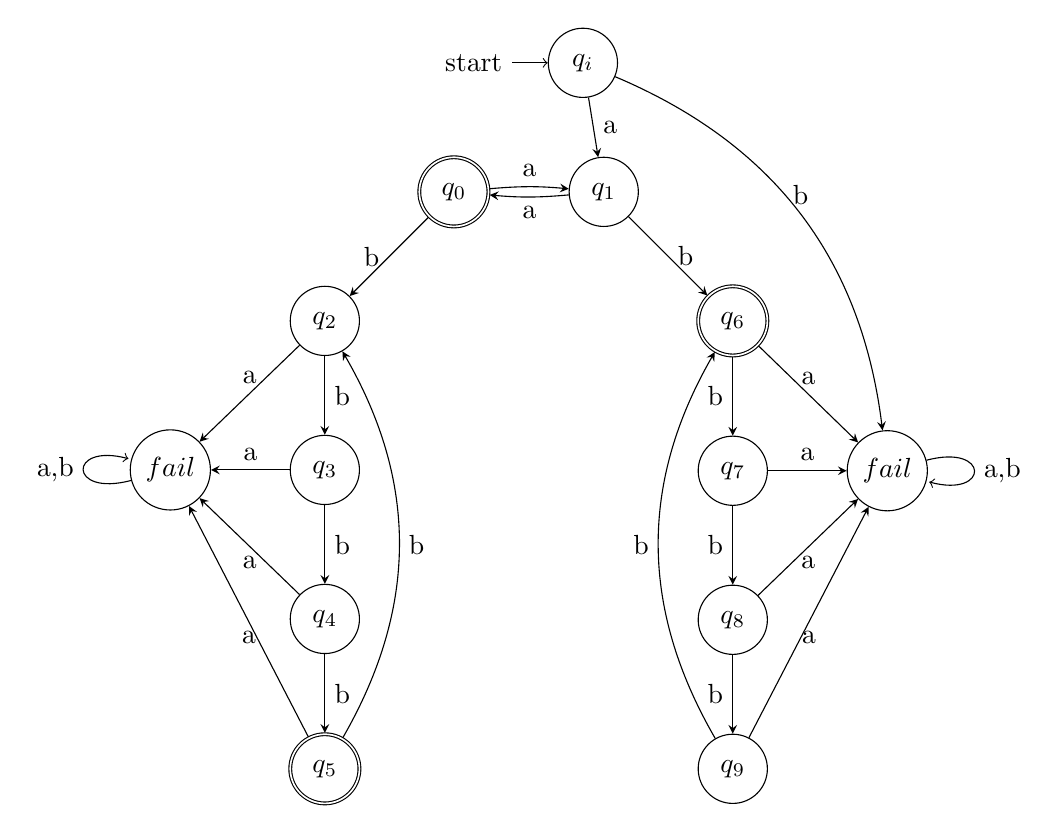
\begin{tikzpicture}
    \node [state, initial] (q_i) {$q_i$};
    \node [state, accepting, below left=of q_i] (q_0) {$q_0$};
    \node [state, right=of q_0] (q_1) {$q_1$};
    \node [state, below left=of q_0] (q_2) {$q_2$};
    \node [state, below=of q_2] (q_3) {$q_3$};
    \node [state, below=of q_3] (q_4) {$q_4$};
    \node [state, accepting, below=of q_4] (q_5) {$q_5$};
    \node [state, accepting, below right=of q_1] (q_6) {$q_6$};
    \node [state, below=of q_6] (q_7) {$q_7$};
    \node [state, below=of q_7] (q_8) {$q_8$};
    \node [state, below=of q_8] (q_9) {$q_9$};
    \node [state, left=of q_3] (q_10) {$fail$};
    \node [state, right=of q_7] (q_11){$fail$};
      \path[->, -stealth]
      (q_0) edge [bend left=5] node [above] {a} (q_1)
      (q_1) edge [bend left=5] node [below] {a} (q_0)
      (q_0) edge node [left] {b} (q_2)
      (q_1) edge node [right] {b} (q_6)
      (q_2) edge node [above] {a} (q_10)
      (q_6) edge node [above] {a} (q_11)
      (q_2) edge node [right] {b} (q_3)
      (q_6) edge node [left] {b} (q_7)
      (q_3) edge node [above] {a} (q_10)
      (q_7) edge node [above] {a} (q_11)
      (q_3) edge node [right] {b} (q_4)
      (q_7) edge node [left] {b} (q_8)
      (q_4) edge node [below] {a} (q_10)
      (q_8) edge node [below] {a} (q_11)
      (q_4) edge node [right] {b} (q_5)
      (q_8) edge node [left] {b} (q_9)
      (q_5) edge node [below] {a} (q_10)
      (q_9) edge node [below] {a} (q_11)
      (q_5) edge [bend right] node [right] {b} (q_2)
      (q_9) edge [bend left] node [left] {b} (q_6)
      (q_i) edge [bend left] node [above] {b} (q_11)
      (q_i) edge node [right] {a} (q_1)
      (q_10) edge [loop left] node [left] {{a,b}} ()
      (q_11) edge [loop right] node [right] {{a,b}} ()
      ;
  \end{tikzpicture}
\end{s}
\section{Models}
\emph{\newline Given the language L above the abc $\{a, b, c\}$, which is defined the folowing way:} \newline
  \emph{$L_1 = \{c^{1+k+n}b^{k}a^{2n} \mid n, k \ge 1\}$} \newline
  \begin{p}
    \emph{\newline Determine what would be the shortest would acceptable by the language:}
  \end{p}
  \begin{s}
    \emph{\newline Should we like for a word to be short, we would be obliged to decrease n and k. Should we like for a word to be of the minimal size, we would have to decrease n and k to their minimums. Thus the value 1 is chosen for n and k and therefore the word is: $c^{1 + 1 + 1}b^{1}a^{2n}$, or in other word: cccbaa} 
  \end{s}
\end{document}
